\documentclass[11pt]{article}
\usepackage[final]{graphicx}
\usepackage{subcaption}
\usepackage[utf8]{inputenc}
\usepackage{listings}
\usepackage{color}
\usepackage{fancyhdr}
\usepackage{enumerate}
\usepackage{enumitem}
\usepackage{hyperref}
\usepackage{wordlike}

% \makeatletter
% \setlength{\@fptop}{0pt}
% \makeatother

% Make hyperlinks prettier
\hypersetup{
    colorlinks=true,
    linkcolor=blue,
    filecolor=magenta,      
    urlcolor=cyan,
}

% Python code formatting
\definecolor{codegreen}{rgb}{0,0.6,0}
\definecolor{codegray}{rgb}{0.5,0.5,0.5}
\definecolor{codepurple}{rgb}{0.58,0,0.82}
\definecolor{backcolour}{rgb}{0.95,0.95,0.92}
 
\lstdefinestyle{mystyle}{
    backgroundcolor=\color{backcolour},
    commentstyle=\color{codegreen},
    keywordstyle=\color{magenta},
    numberstyle=\tiny\color{codegray},
    stringstyle=\color{codepurple},
    basicstyle=\small,
    breakatwhitespace=false,
    breaklines=true,
    captionpos=t,
    keepspaces=true,
    numbers=left,
    numbersep=5pt,
    showspaces=false,
    showstringspaces=false,
    showtabs=false,
    tabsize=2
}

\lstset{style=mystyle}

\setlist{parsep=0pt,listparindent=\parindent}

% Header settings  
\pagestyle{fancy}
\fancyhf{}
\rhead{10/06/2016}
\chead{Paul Ruess}
\lhead{CE 385S -- Homework 3}
\rfoot{Page \thepage}

\begin{document}

\section*{\centerline{Homework 3 -- Problem 4}}

The Height Above Nearest Drainage (HAND) methodology has recently been adopted by Xing Zheng and Dr. David Maidment at the University of Texas at Austin to improve flood inundation mapping efforts; this is done by generalizing National Elevation Dataset (NED) grid-cells (10m x 10m) as the height above their nearest drainage location (found by following a cell down the path of steepest descent until intersecting with the bottom of a stream reach). The HAND method is relevant to this project because of the data outputs it provides: stream variables (particularly wetted area, hydraulic radius, and slope), and the resulting rating curves derived from these hydraulic properties, can be used to compare the computed HAND rating curves with the ``correct'' United States Geological Survey (USGS) rating curves. Of note, the current HAND rating curves are determined assuming a manning's $n$ of 0.05 for all stream reaches (see equation 1); this is the motivation for this study -- I would like to programmatically determine what the ``correct'' manning's $n$ should be on a large scale, and perhaps statistically compare these corrected $n$ values to the 0.05 assumption currently used. 

\begin{equation}
Q = \frac{k}{n}AR^\frac{2}{3}S^\frac{1}{2}
\end{equation}
where: 
\begin{description}
\item[Q] is the discharge (L\textsuperscript{3}/T; ft/s, m/s);
\item[A] is the cross-sectional area (L\textsuperscript{2}; ft\textsuperscript{2}, m\textsuperscript{2});
\item[R] is the hydraulic radius (L; ft, m);
\item[S] is the channel bed slope at constant water depth (L/L, ft/ft, m/m).
\item[k] is a conversion factor, 1.0 for SI units and 1.49 for English units.
\end{description}

\vspace{1ex}

In short, this project has changed to become more of a statistical curve-fitting of  HAND rating curves to USGS rating curves. The intent is to programmatically snap a HAND rating curve to the USGS rating curve; this involves a statistical optimization of sorts (I'm still figuring this part out) including an adjustment of the HAND rating curve to the USGS stream bottom depth (which itself requires adjustment), and a subsequent fitting of the HAND rating curve to the USGS rating curve by adjusting manning's $n$ (roughness). The first step, then, requires collection of the actual data: USGS rating curves were collected online (ex: \url{http://waterdata.usgs.gov/nwisweb/get_ratings?file_type=exsa&site_no=08158810}, where the last eight digits are the USGS identifier), and HAND rating curves and hydrologic information were received from Xing Zheng for the Onion Creek watershed in Austin, Texas. Onion Creek will be used as an initial test case, with the intent of expanding the final rating curve optimization scheme to all of Texas (and, eventually, all of the United States). \\

% \clearpage

After the data was collected, a preliminary assessment was conducted in which the ``correct'' manning's $n$ for each of eight stream reaches within the Onion Creek watershed were manually determined. Figures 1a through 1h (see pages 3 and 4) show both the HAND rating curves (red), the USGS rating curves (blue), and the HAND rating curve after it has been manually fitted to the USGS rating curve (green); the manning's $n$ value displayed in the upper right-hand corner of each image is the roughness that was used for the fit. \\

The first thing that is evident is that the ``correct'' manning's $n$ values are quite high. As seen in the following url: \url{http://www.fsl.orst.edu/geowater/FX3/help/8_Hydraulic_Reference/Mannings_n_Tables.htm}, manning's $n$ is generally between 0.02 and 0.07, with values rarely getting above 0.2. As such, I will need to spend some time reviewing the Python script I am using (Listing 1) to be certain that my mathematical approach and units are correct. Once I am certain that the mathematics is correct, I will proceed to automate the curve fitting. 

\begin{figure}[b!]
\makebox[\linewidth][c]{
\begin{subfigure}{0.65\textwidth}
  \centering
  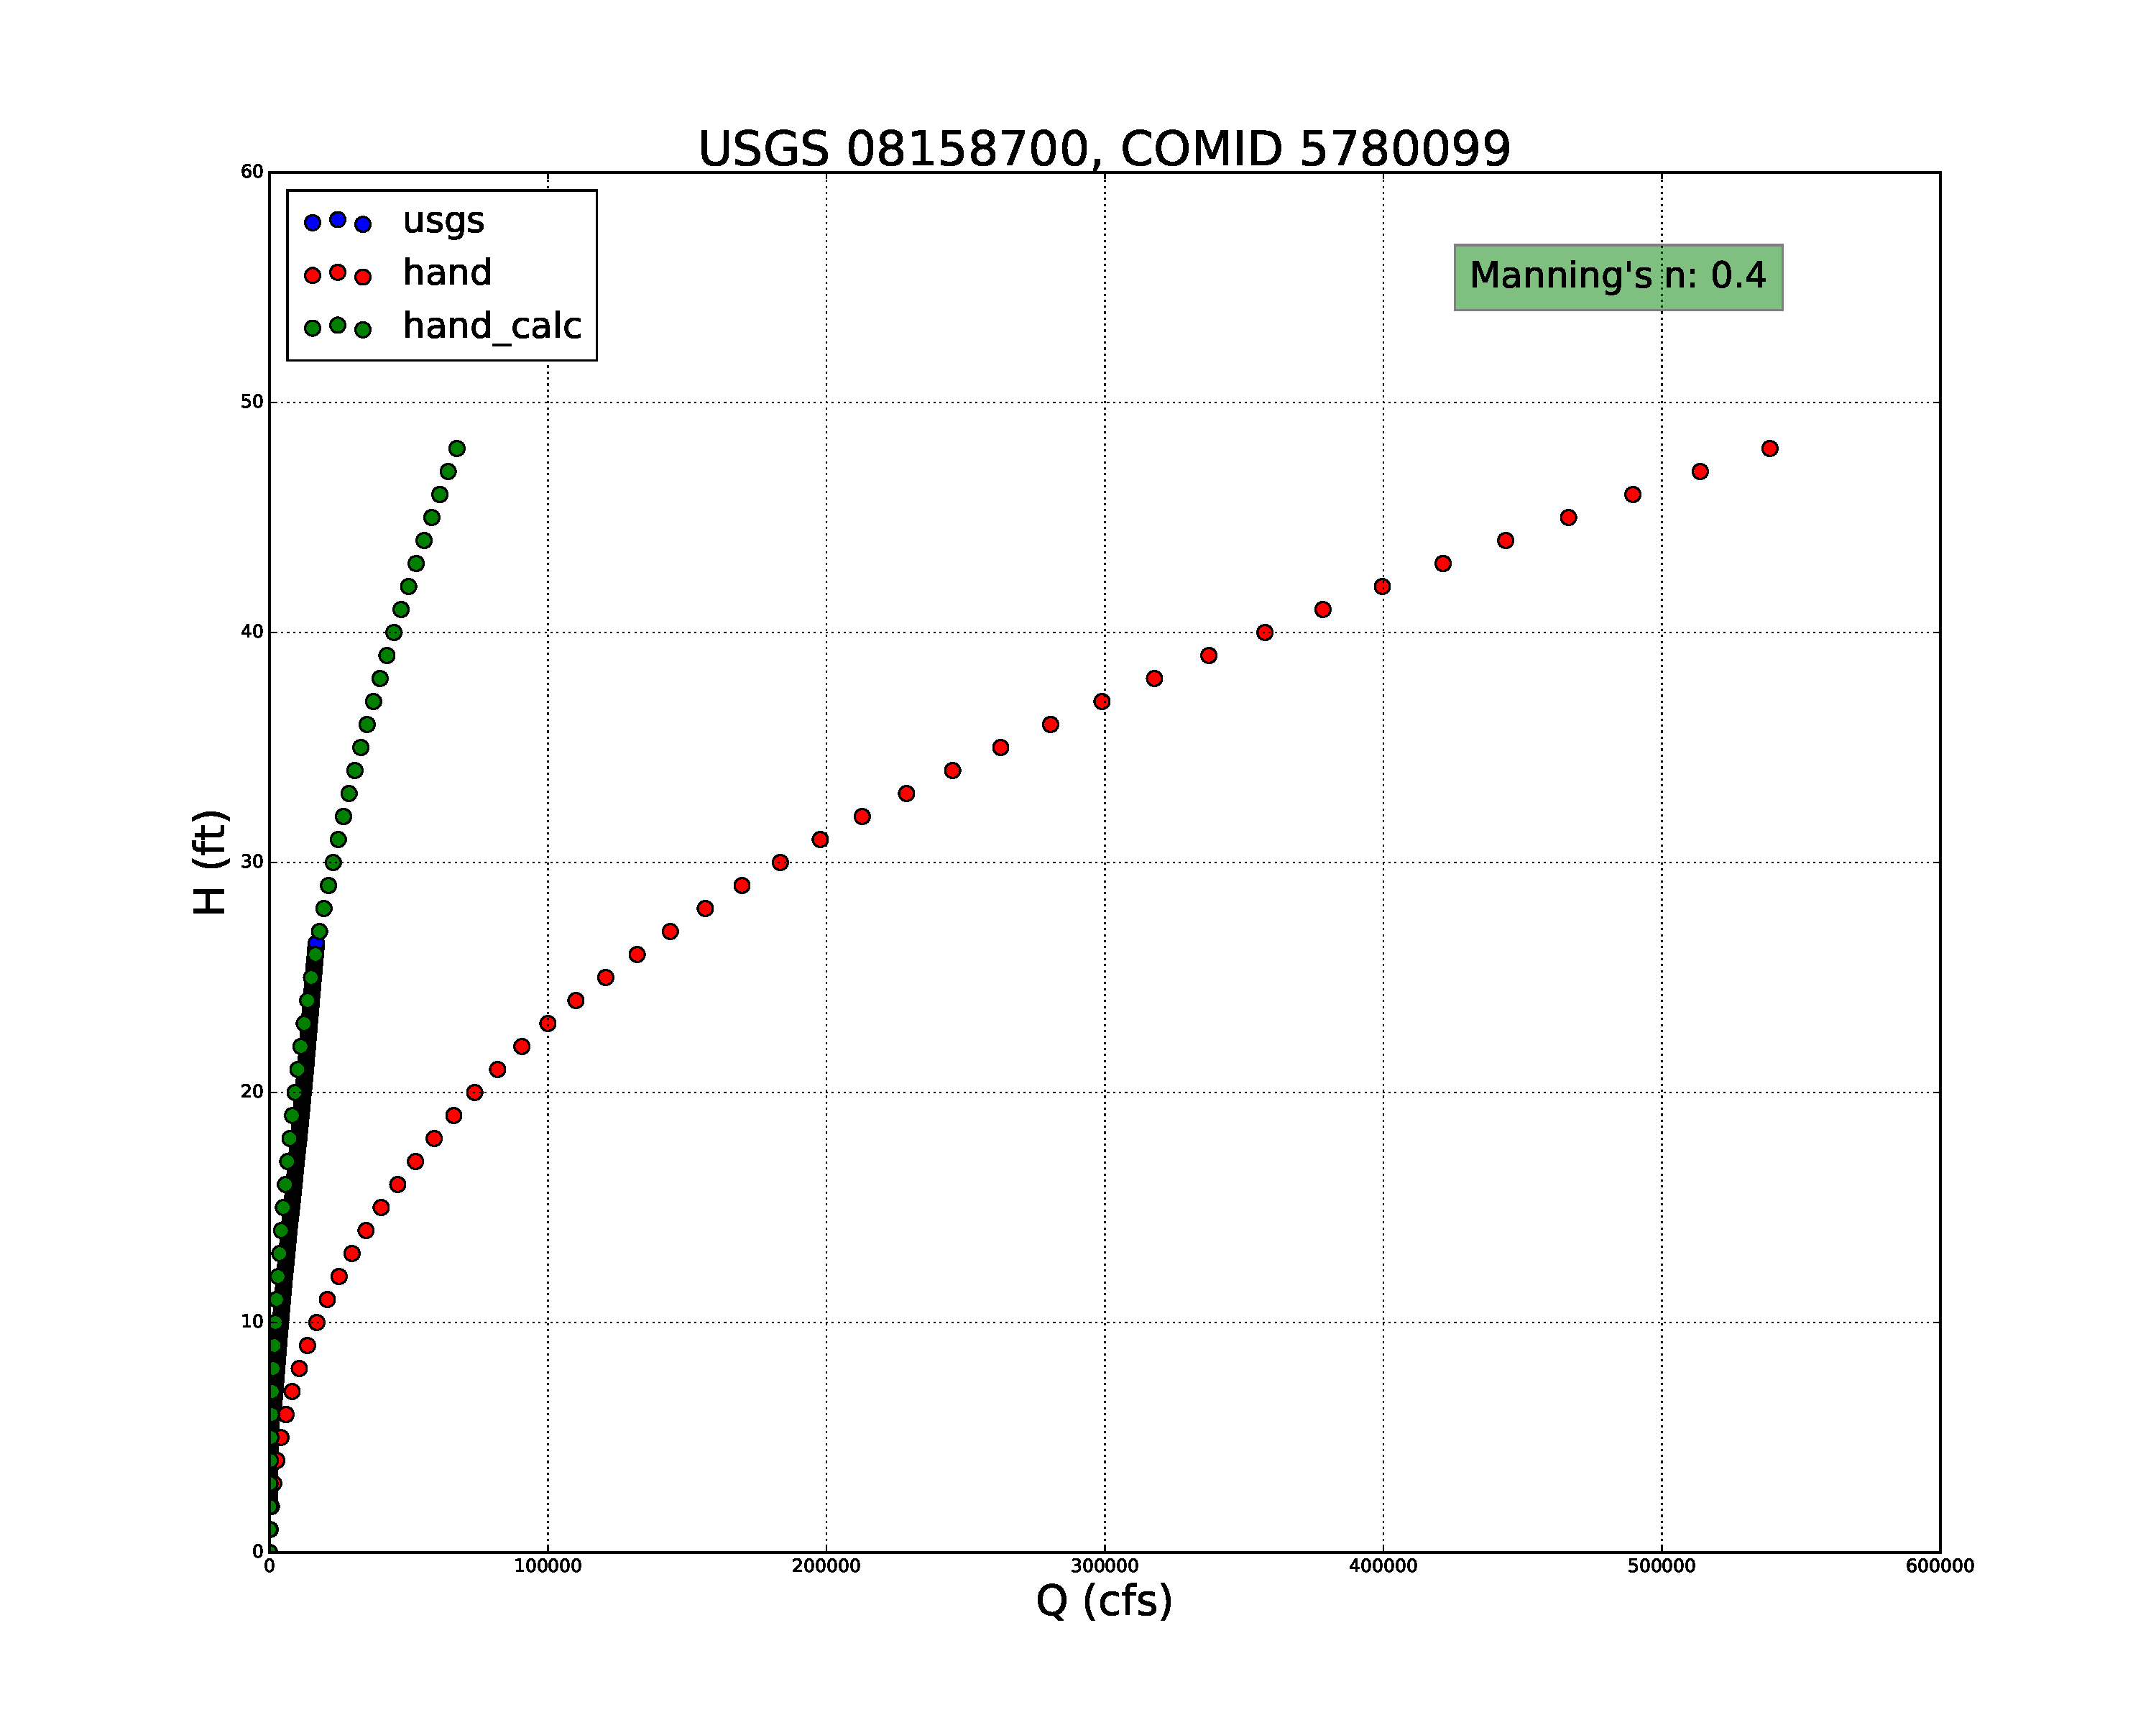
\includegraphics[width=\linewidth]{manualresults/rc_comid_5780099.pdf}
  \caption{Rating Curve for COMID 5780099}\label{fig:a}
\end{subfigure}\hspace*{\fill}
\begin{subfigure}{0.65\textwidth}
  \centering
  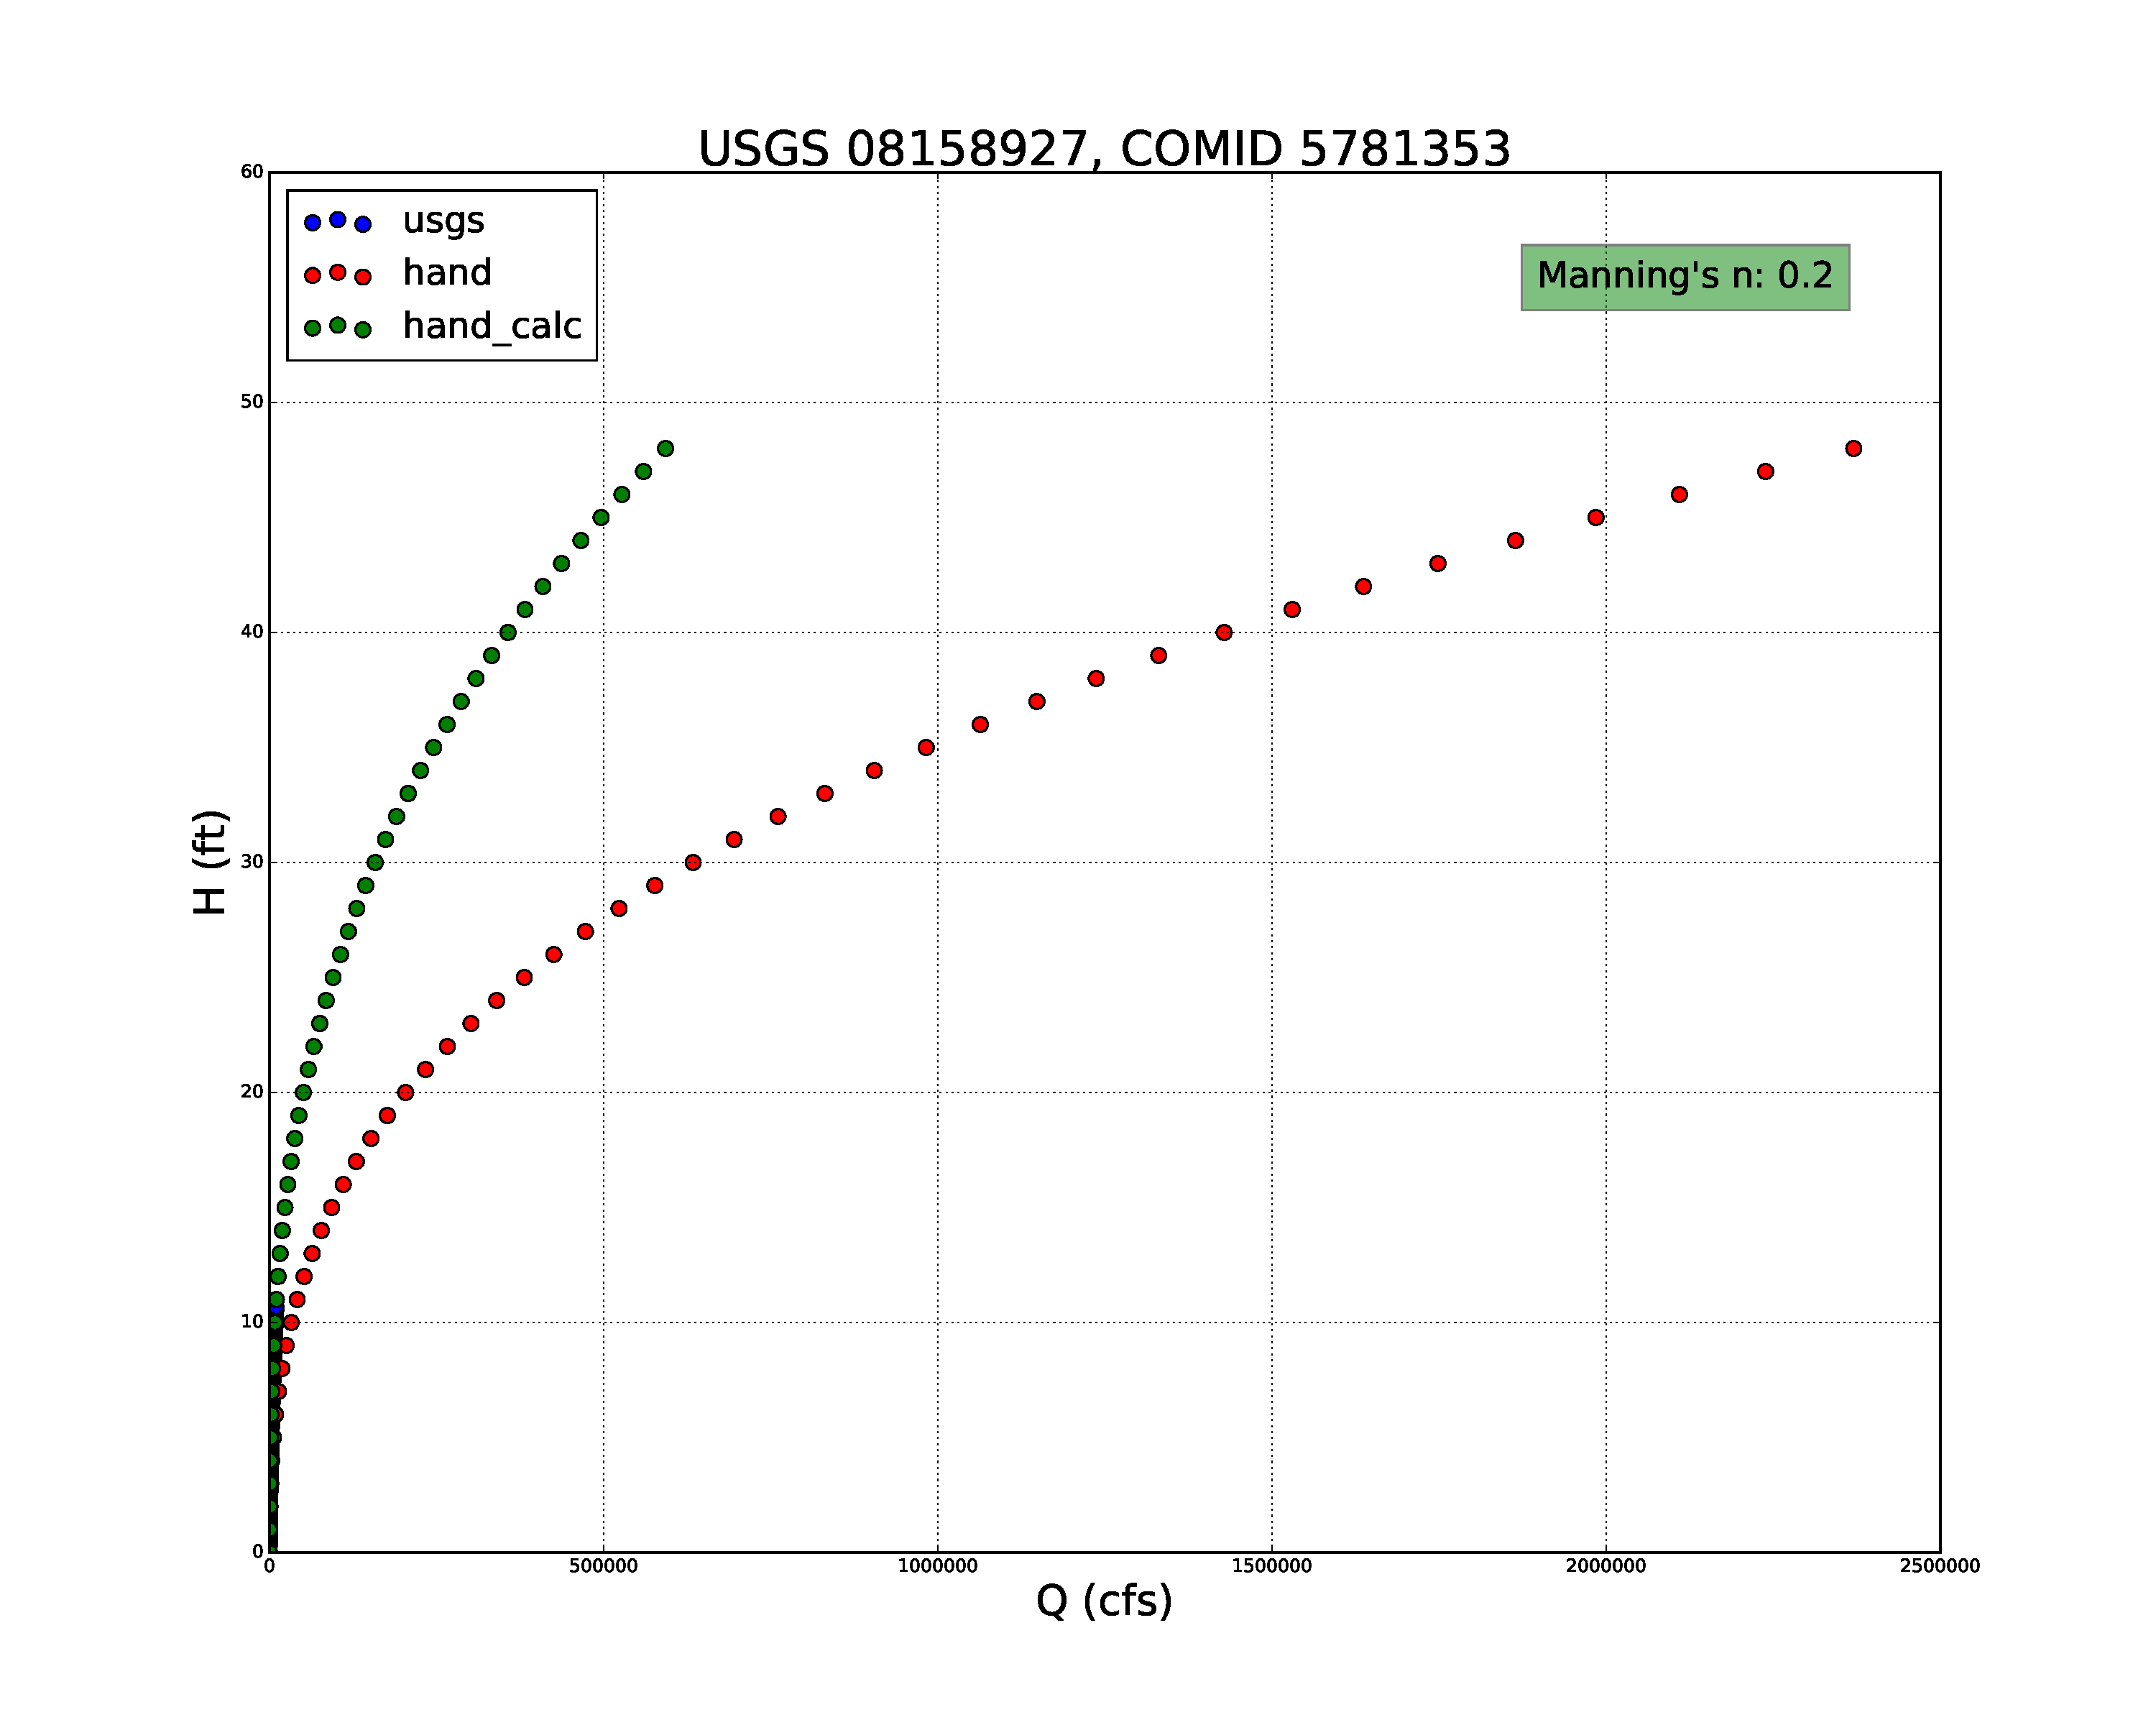
\includegraphics[width=\linewidth]{manualresults/rc_comid_5781353.pdf} \caption{Rating Curve for COMID 5781353}\label{fig:b}
\end{subfigure}\hspace*{\fill}
}

\smallskip
\makebox[\linewidth][c]{
\begin{subfigure}{0.65\textwidth}
  \centering
  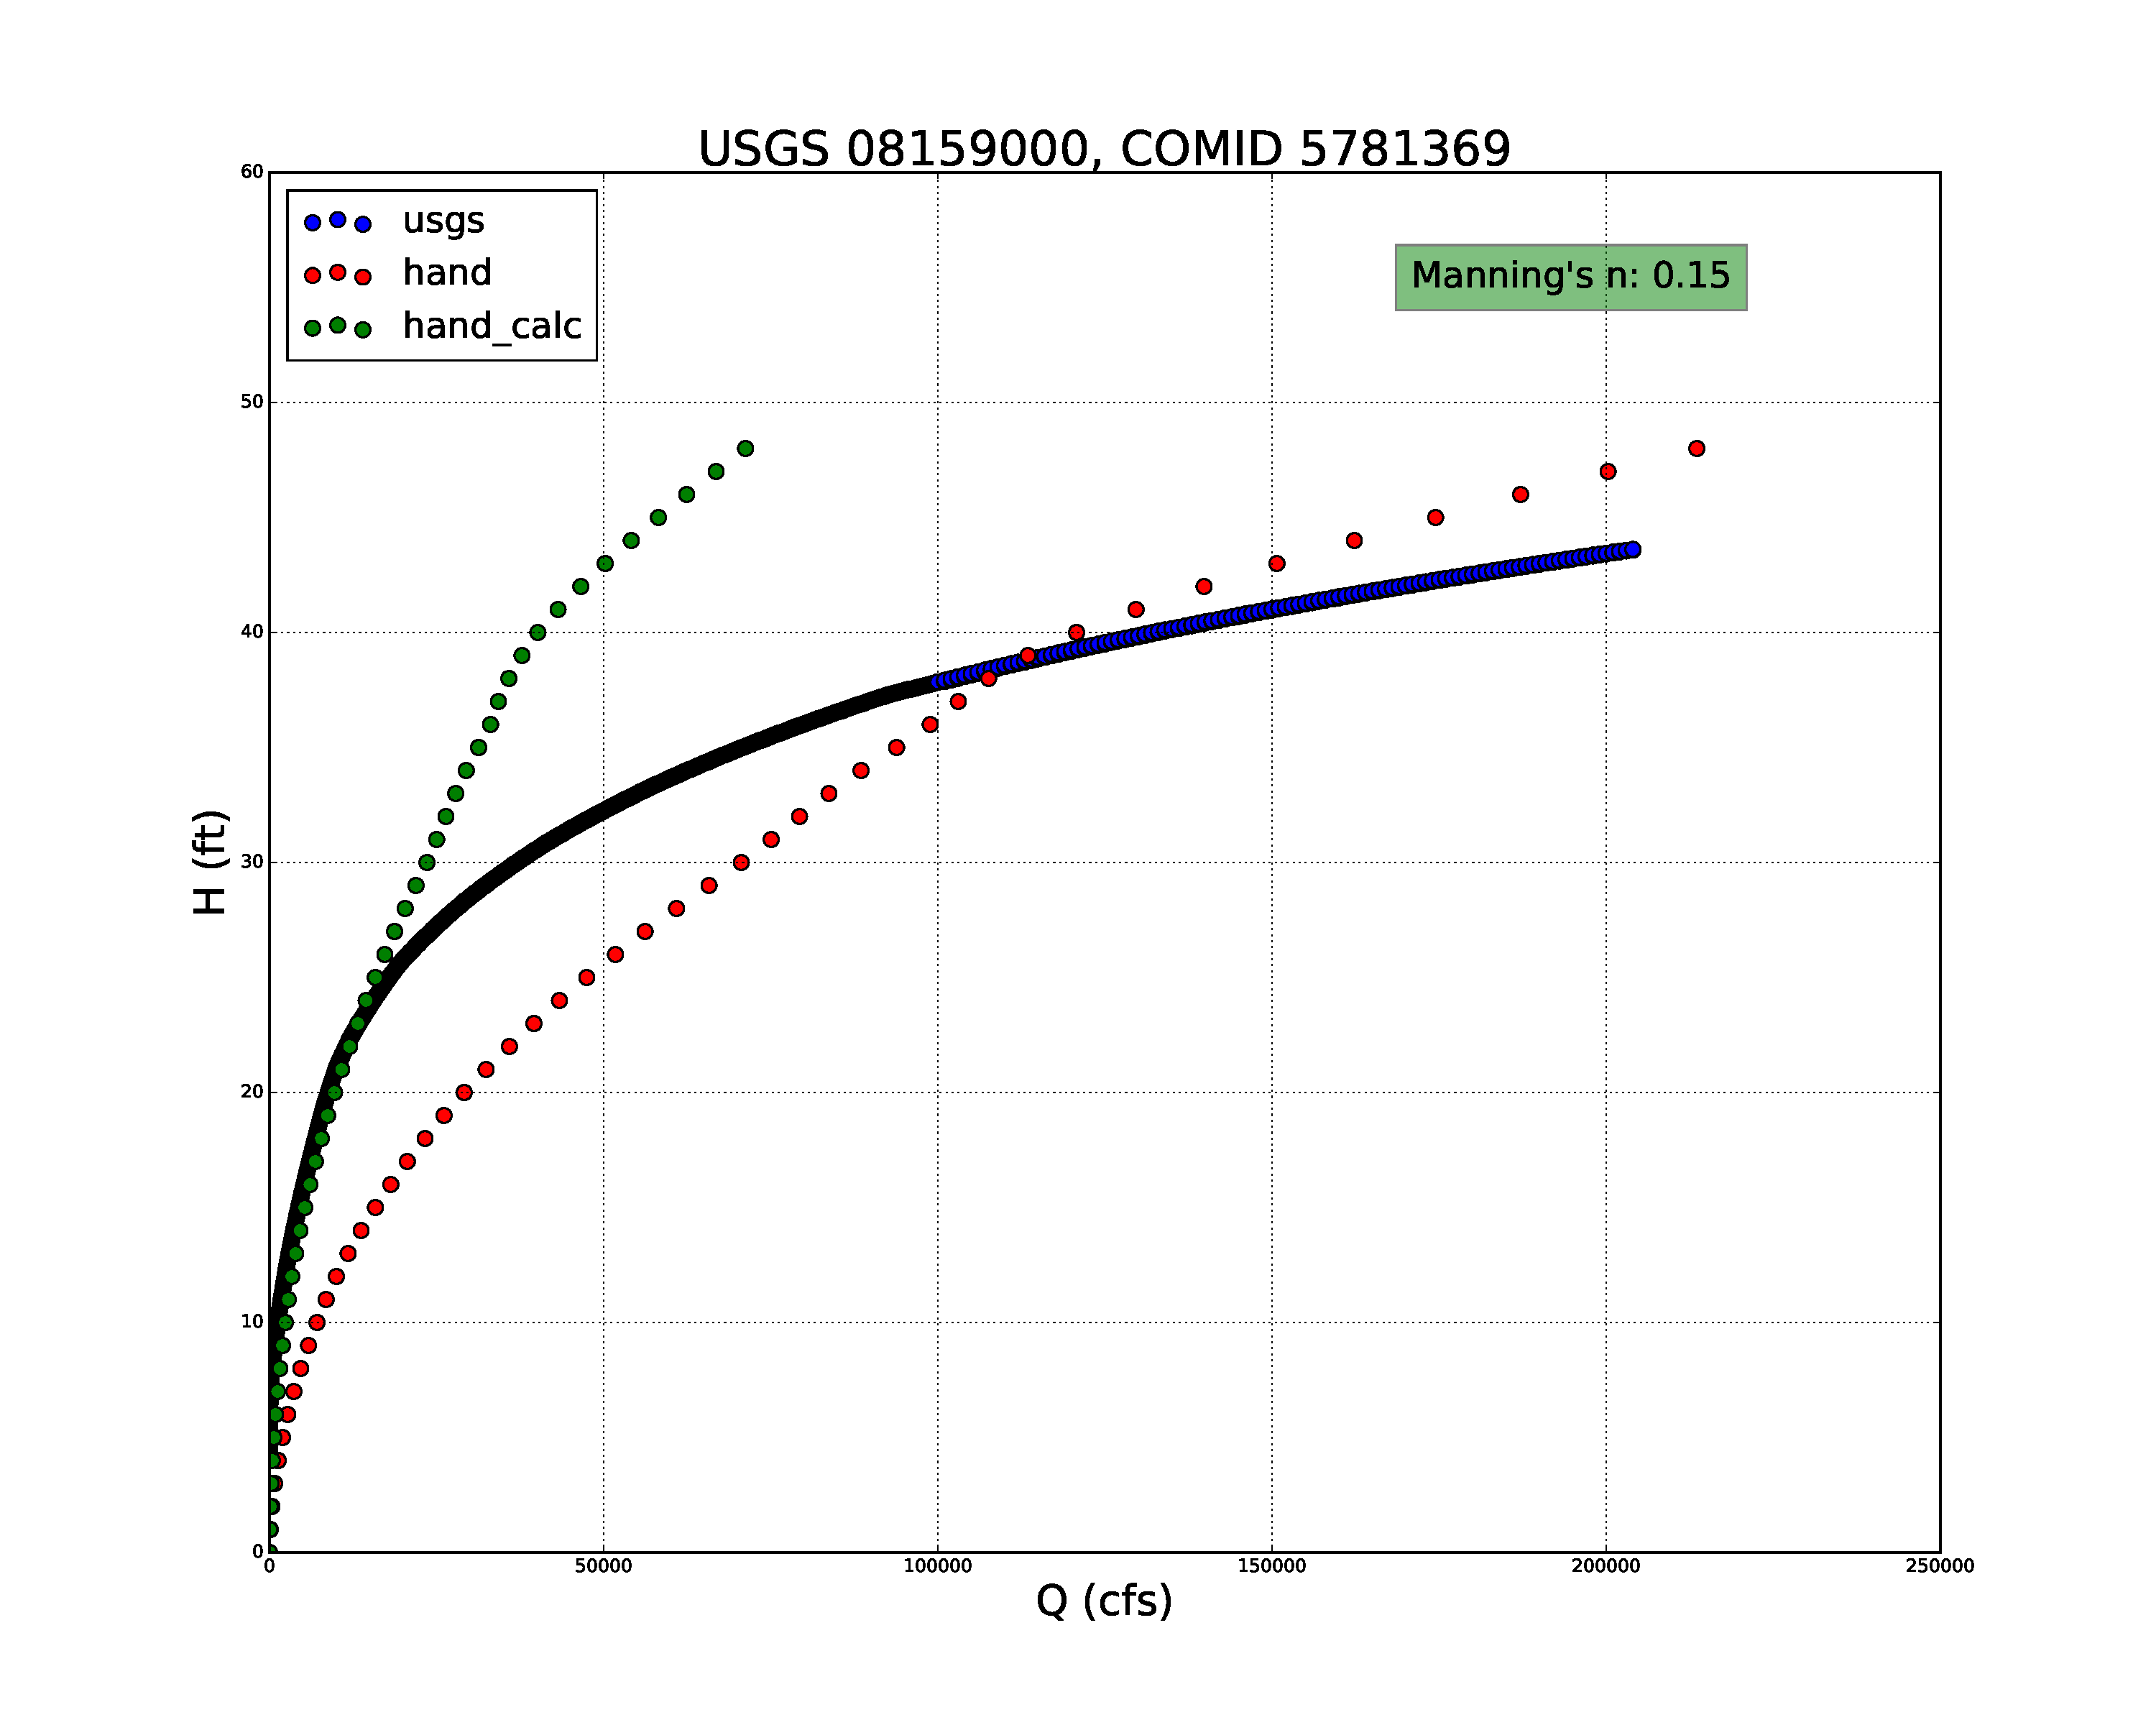
\includegraphics[width=\linewidth]{manualresults/rc_comid_5781369.pdf}
  \caption{Rating Curve for COMID 5781369}\label{fig:c}
\end{subfigure}\hspace*{\fill}
\begin{subfigure}{0.65\textwidth}
  \centering
  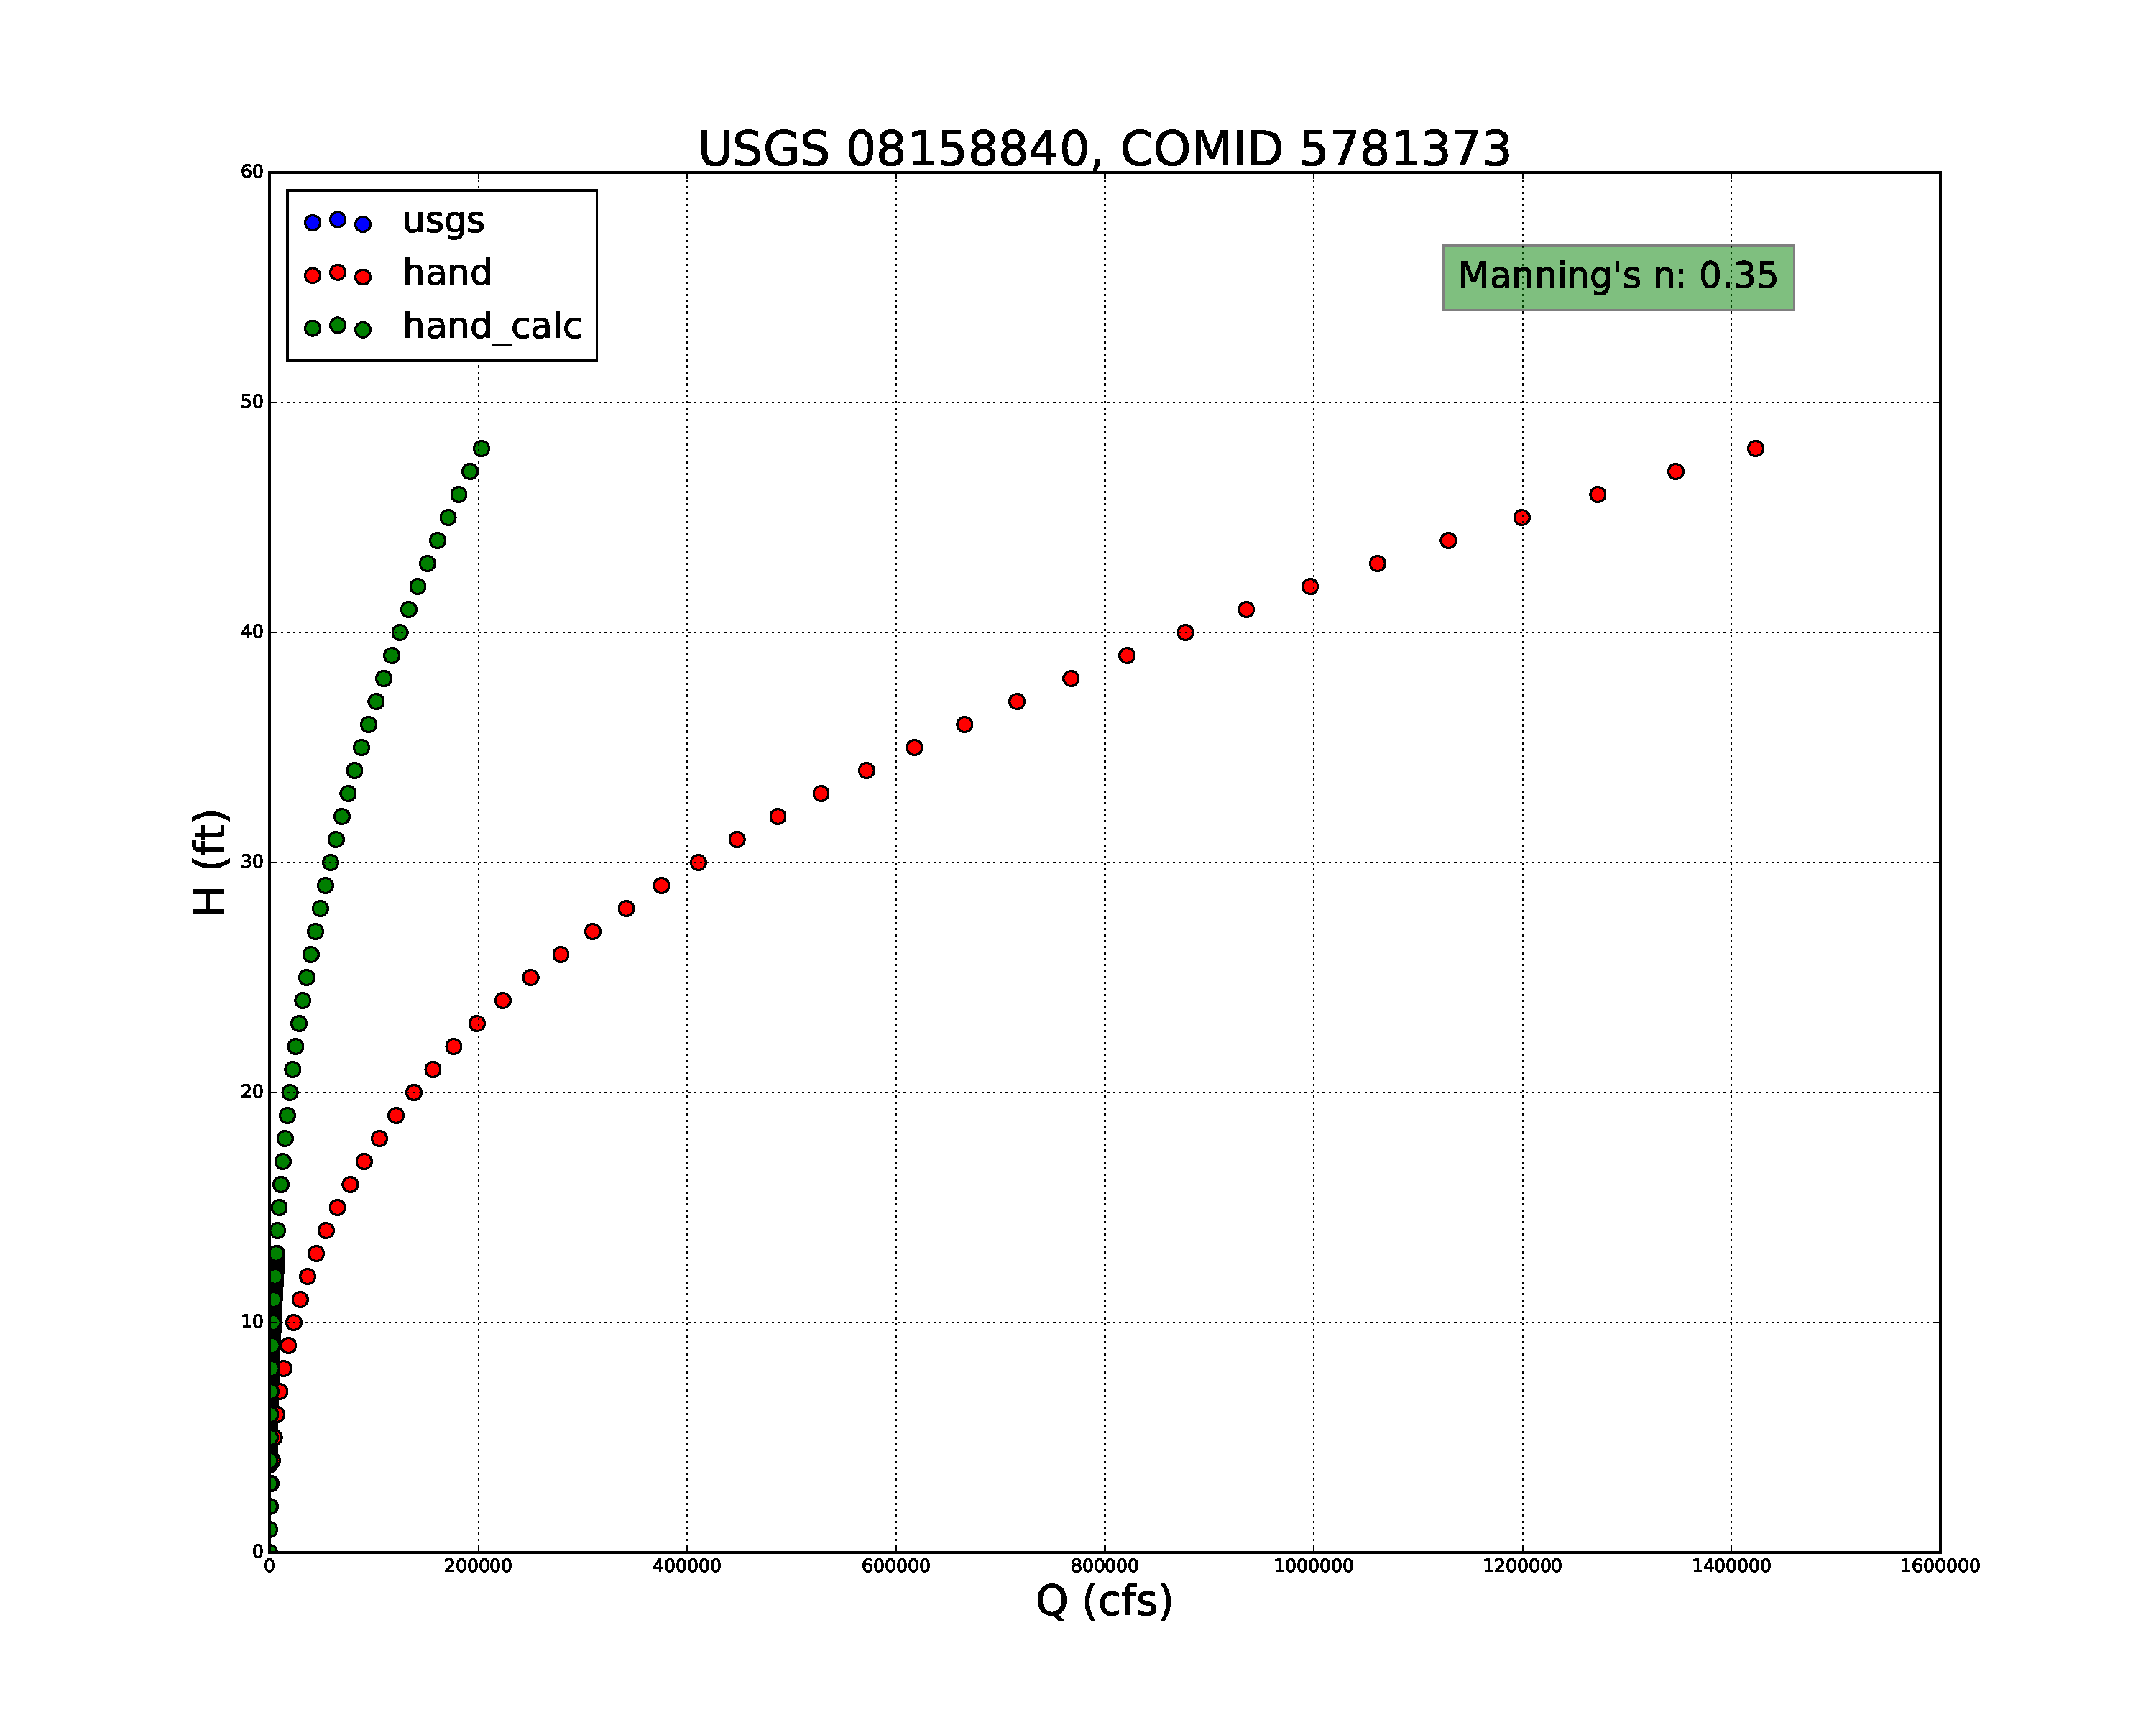
\includegraphics[width=\linewidth]{manualresults/rc_comid_5781373.pdf}
  \caption{Rating Curve for COMID 5781373}\label{fig:d}
\end{subfigure}\hspace*{\fill}
}

\caption{Rating Curves for the Onion Creek watershed in Austin, Texas} \label{fig:1}
\end{figure}

\begin{figure}[b!]
\ContinuedFloat
\makebox[\linewidth][c]{
\begin{subfigure}{0.65\textwidth}
  \centering
  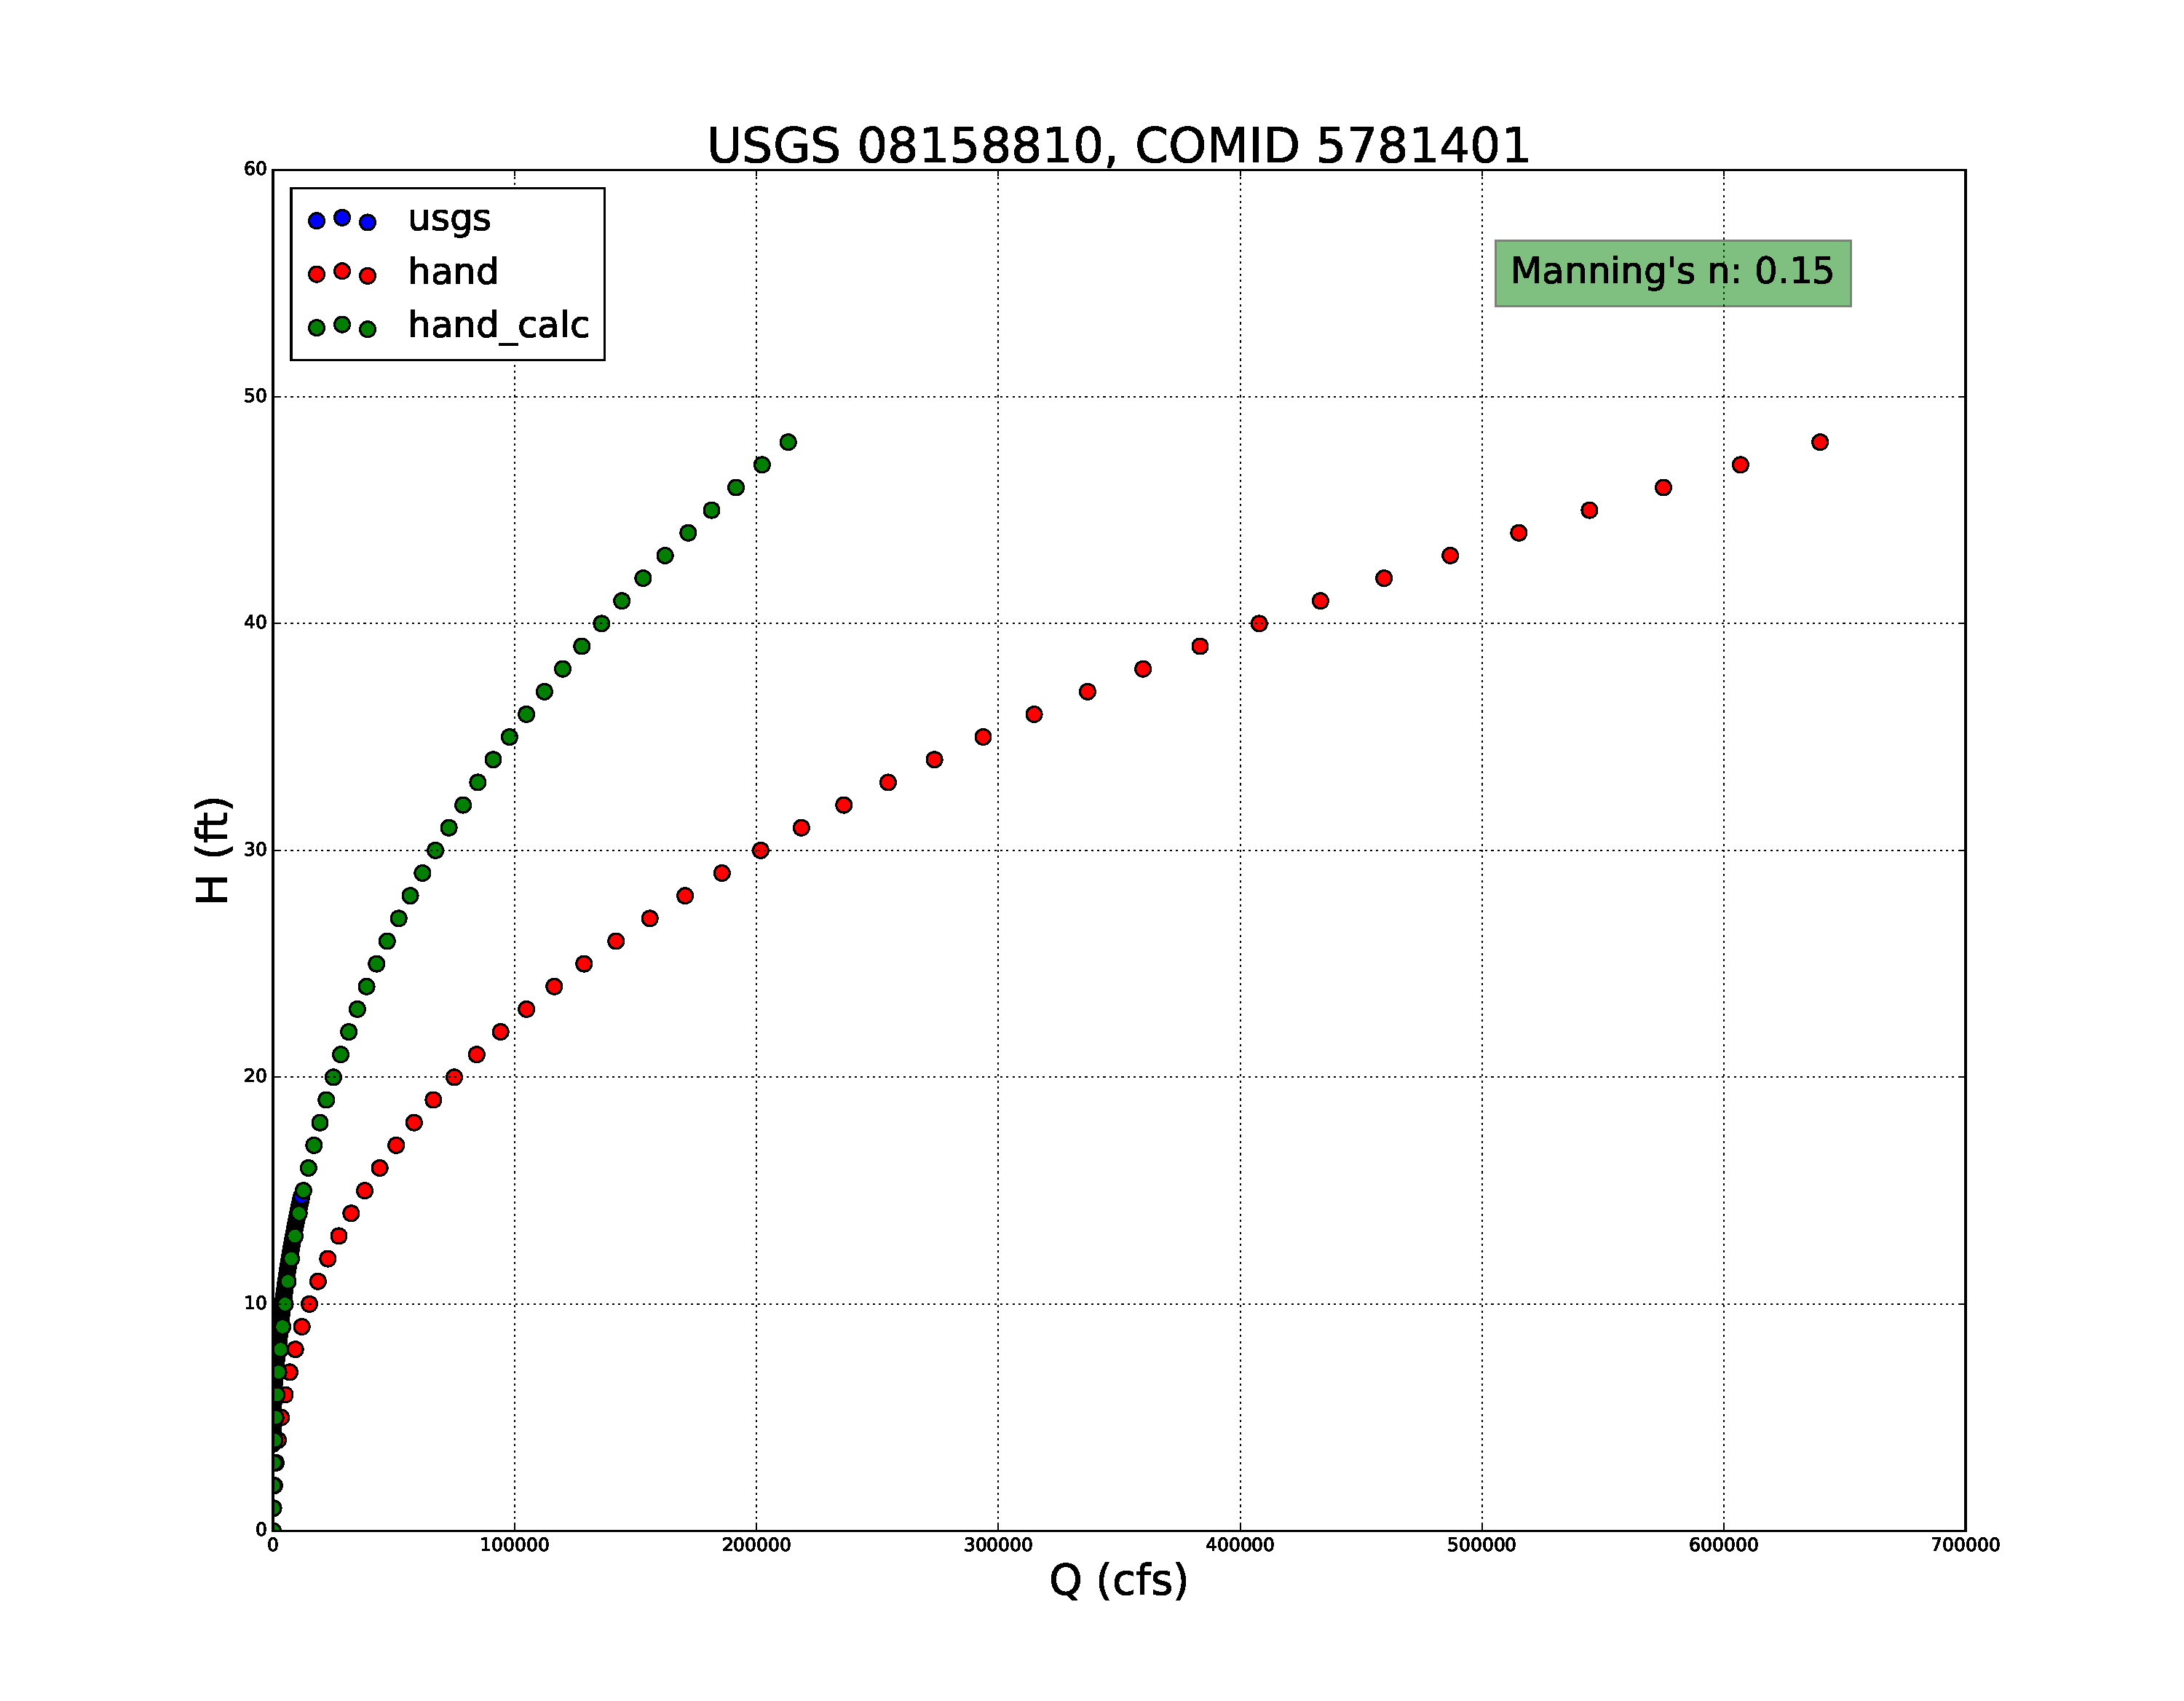
\includegraphics[width=\linewidth]{manualresults/rc_comid_5781401.pdf}
  \caption{Rating Curve for COMID 5781401}\label{fig:e}
\end{subfigure}\hspace*{\fill}
\begin{subfigure}{0.65\textwidth}
  \centering
  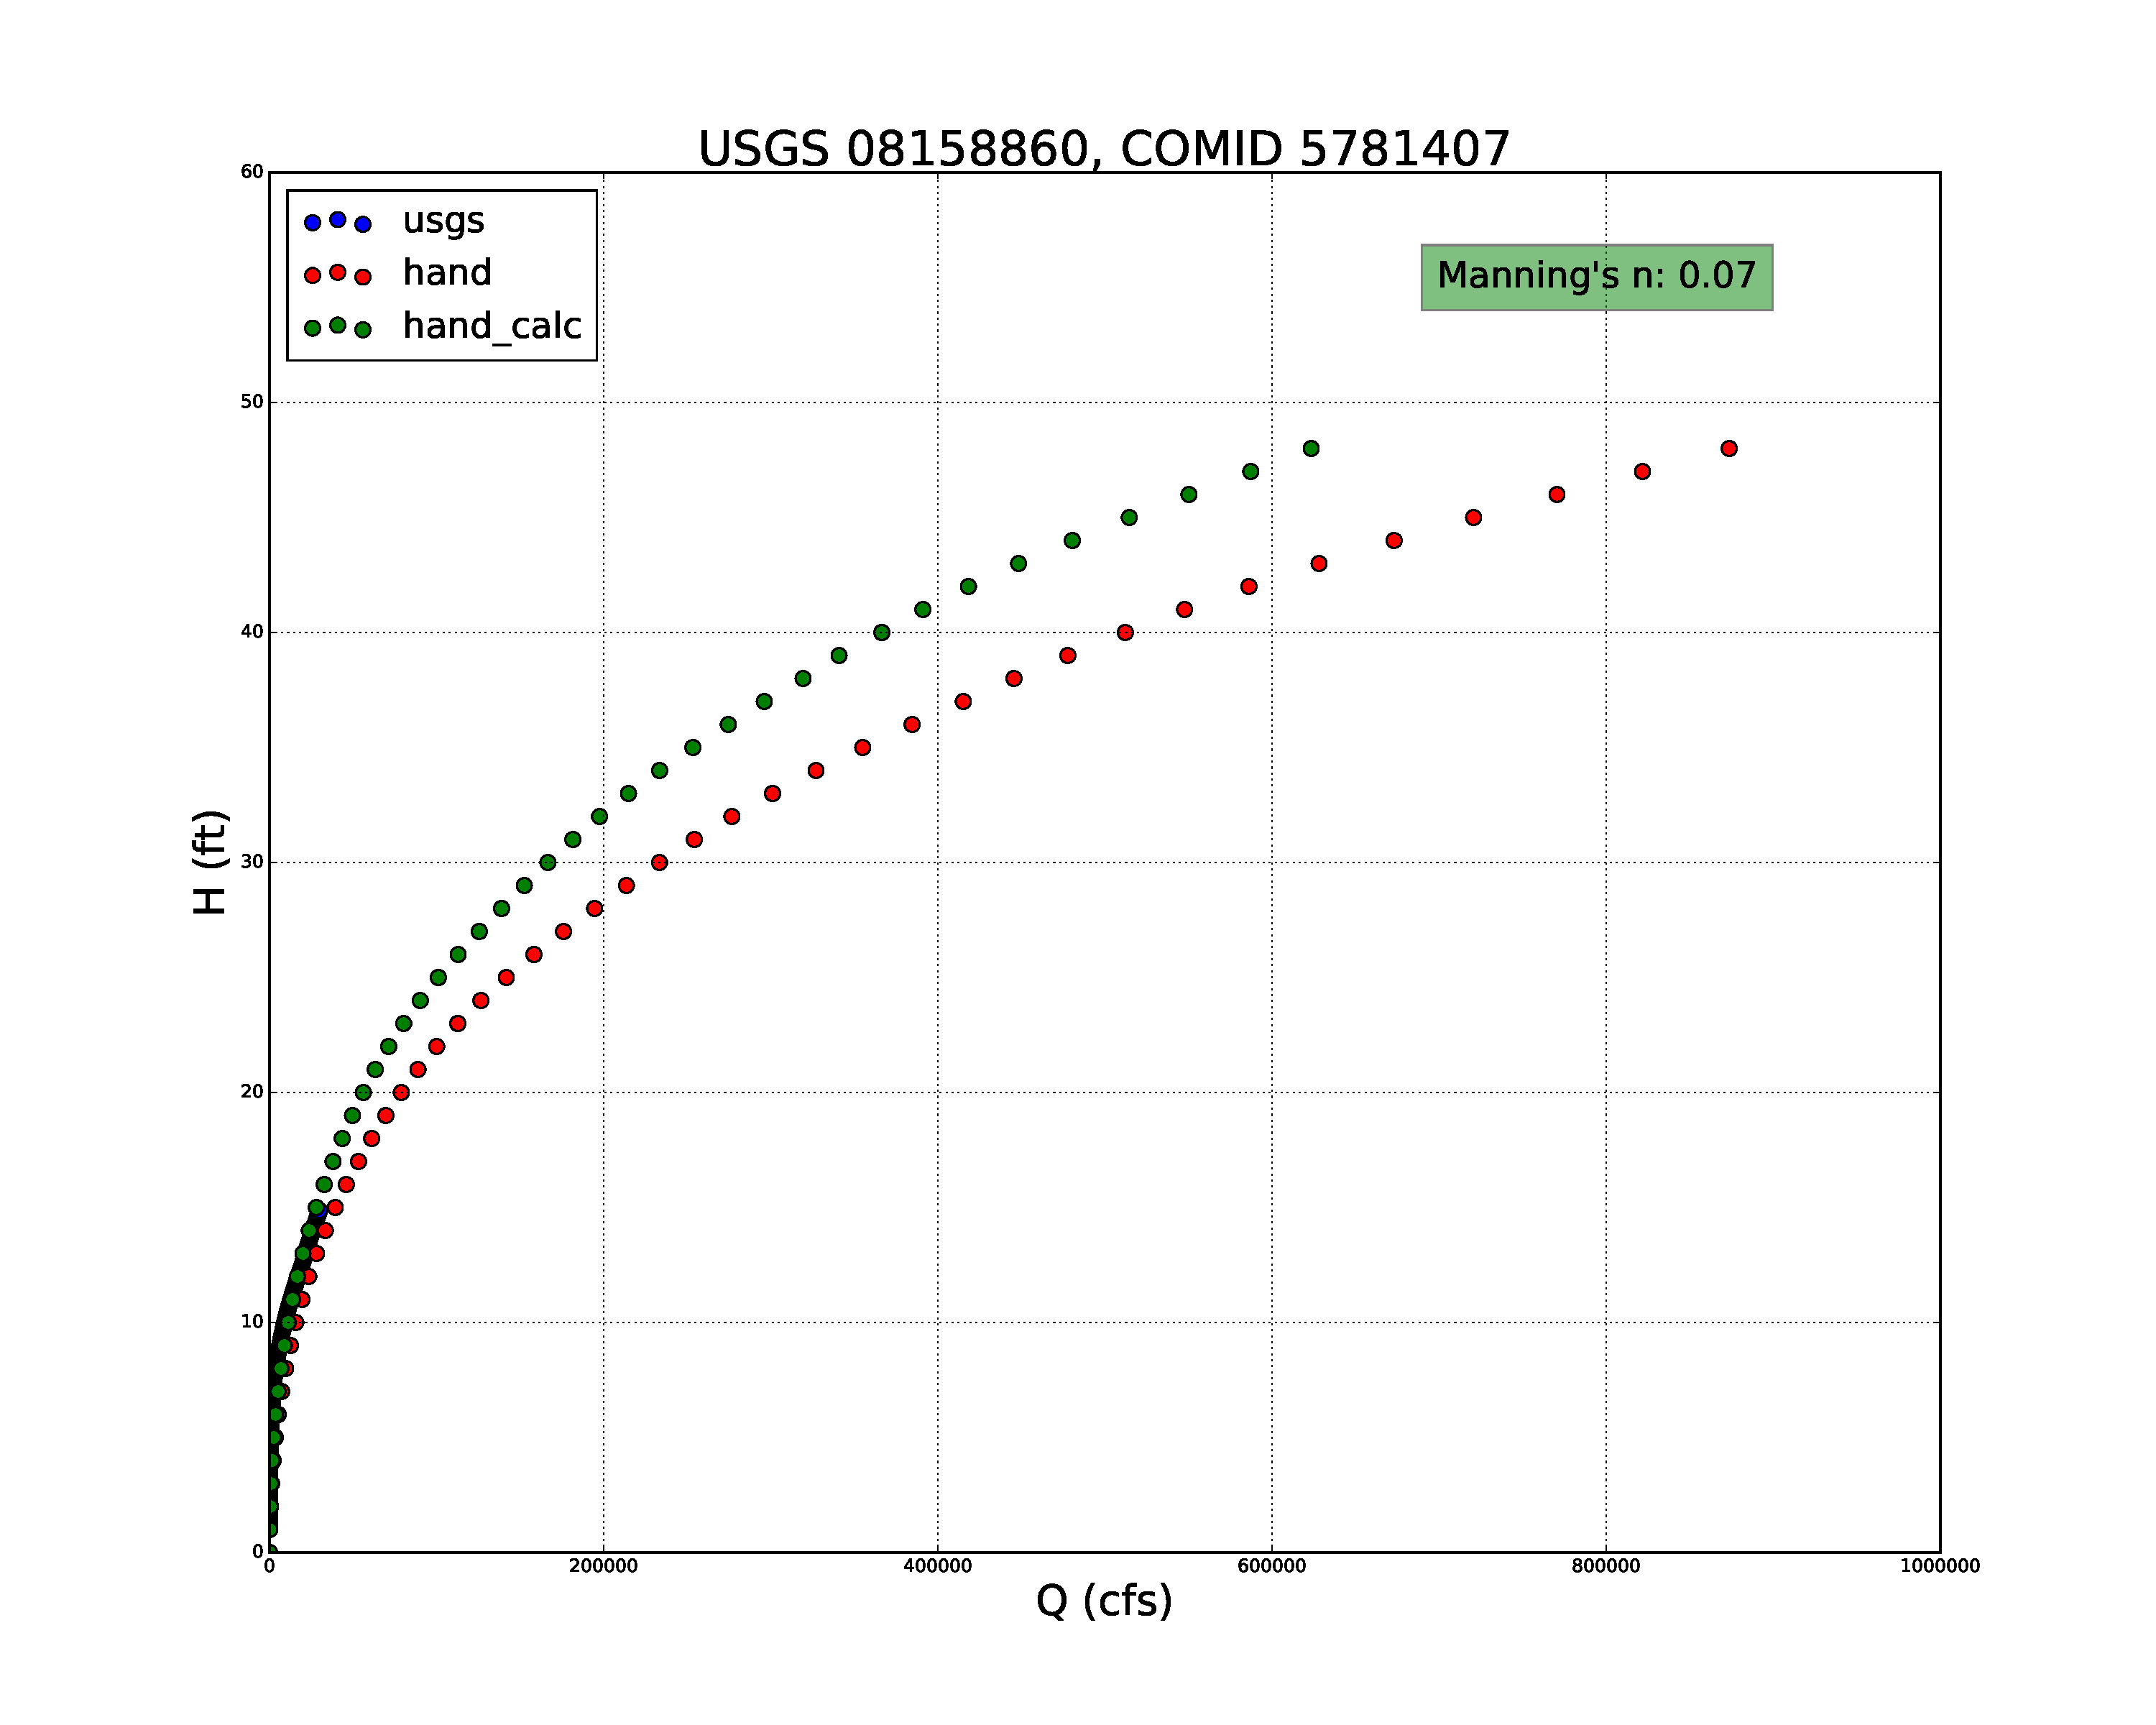
\includegraphics[width=\linewidth]{manualresults/rc_comid_5781407.pdf}
  \caption{Rating Curve for COMID 5781407}\label{fig:f}
\end{subfigure}\hspace*{\fill}
}

\smallskip
\makebox[\linewidth][c]{
\begin{subfigure}{0.65\textwidth}
  \centering
  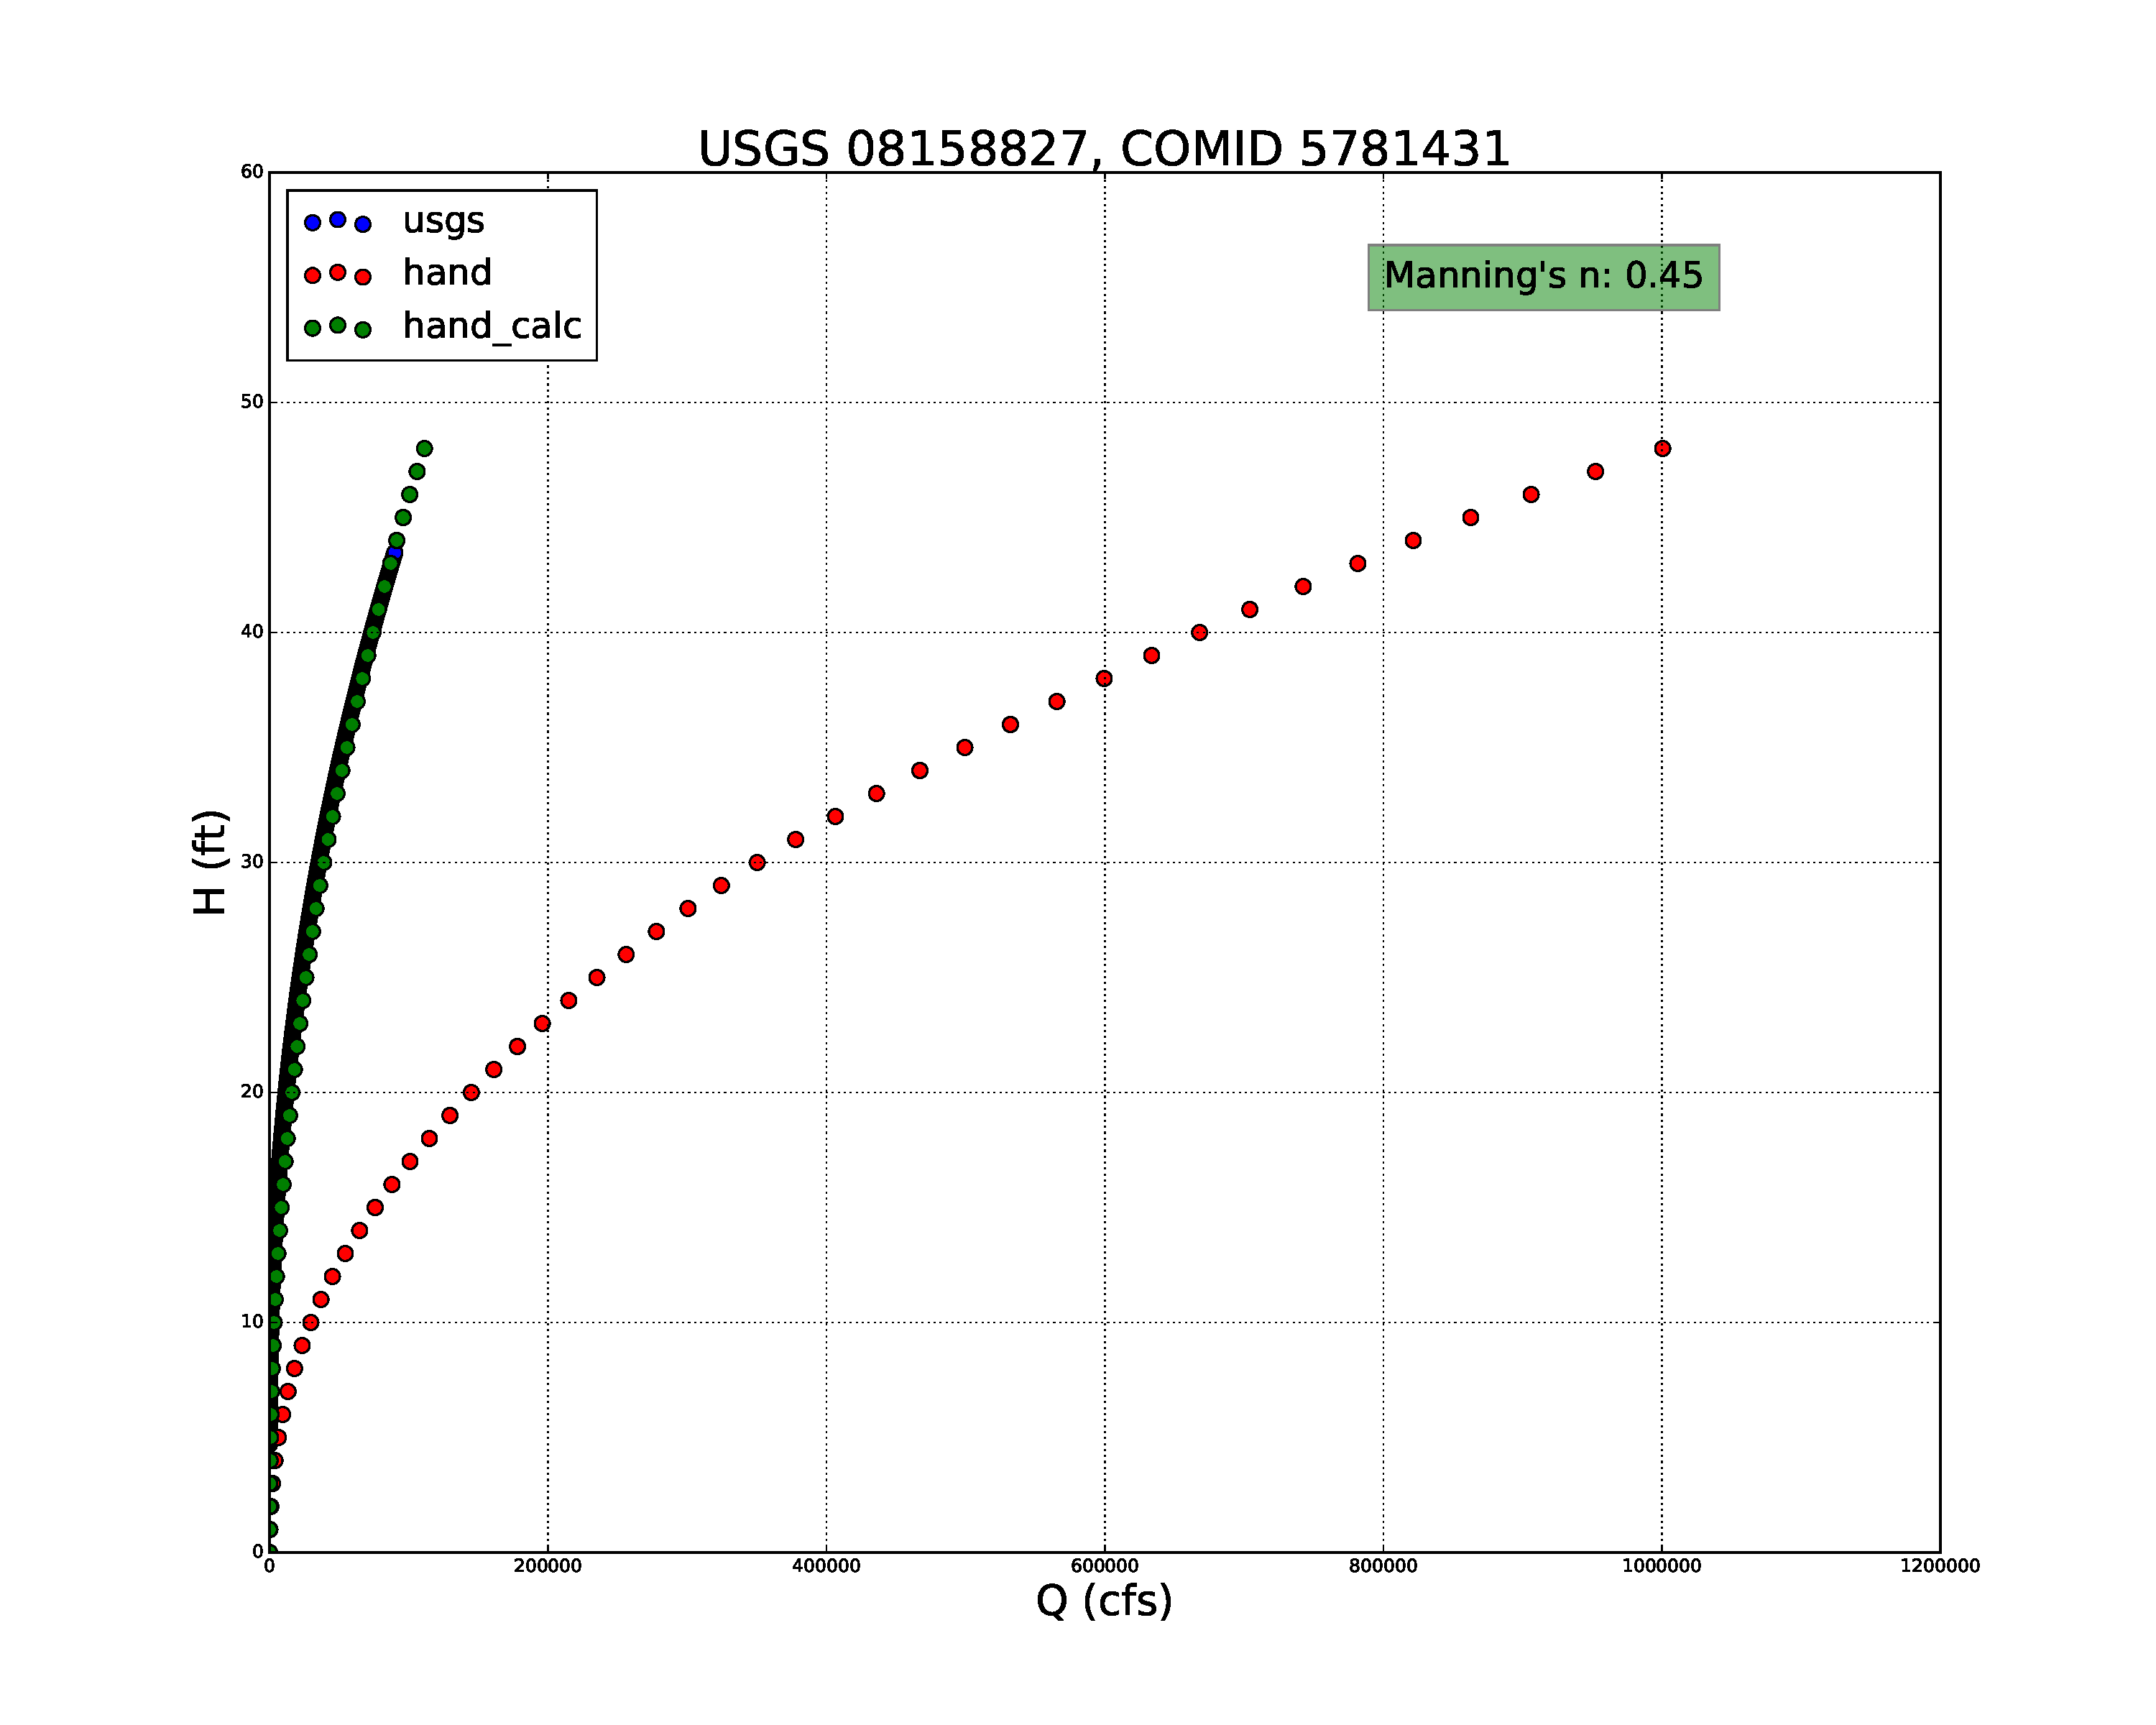
\includegraphics[width=\linewidth]{manualresults/rc_comid_5781431.pdf}
  \caption{Rating Curve for COMID 5781431}\label{fig:g}
\end{subfigure}\hspace*{\fill}
\begin{subfigure}{0.65\textwidth}
  \centering
  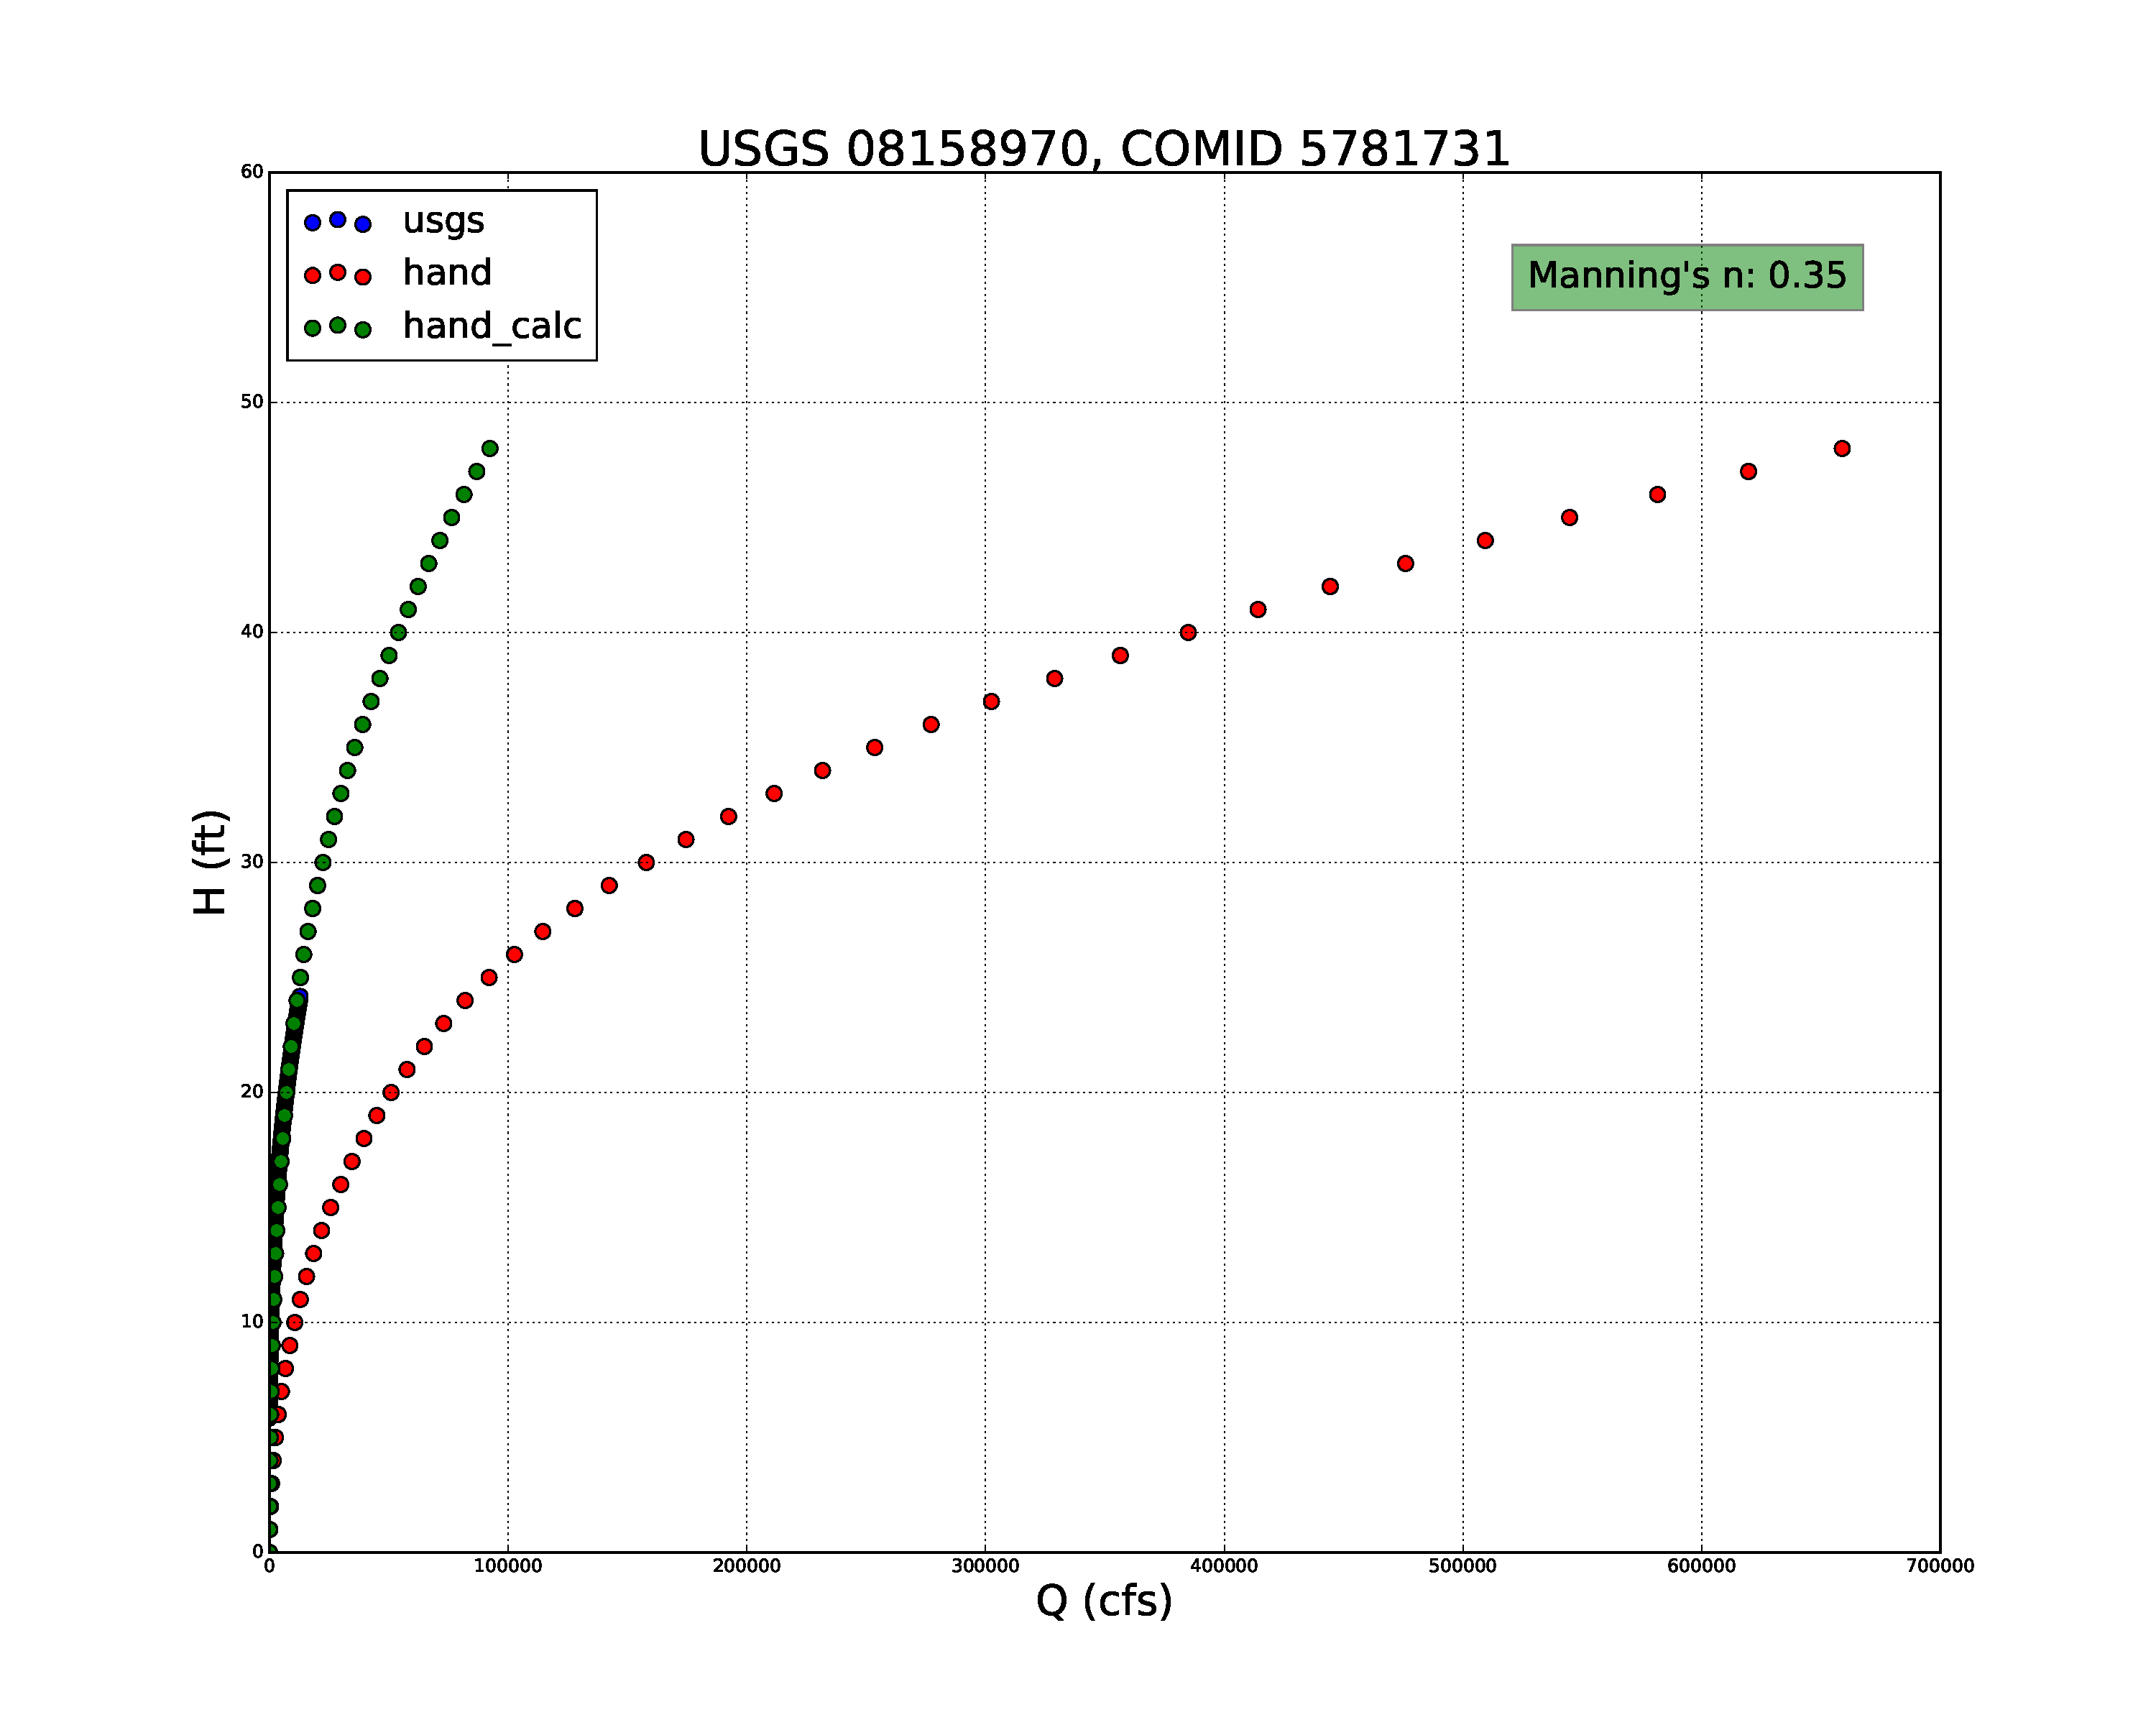
\includegraphics[width=\linewidth]{manualresults/rc_comid_5781731.pdf}
  \caption{Rating Curve for COMID 5781731}\label{fig:h}
\end{subfigure}\hspace*{\fill}
}

\caption{Rating Curves for the Onion Creek watershed in Austin, Texas} \label{fig:1}
\end{figure}

\clearpage

\noindent
Regarding the automation of the curve fitting, there are two main steps: 

\begin{enumerate}
  \item Adjust HAND rating curve to fit USGS rating curve along the y-axis (Height, ft) to correct for the USGS accepted bank bottom. I am still devising the solution to this problem, but -- after taking into account the vertical ``shift'' -- I believe I will need to find the highest depth associated with a discharge of zero (USGS rating curves often have many depths with Q = 0, including depths up to multiple feet high) and then set that height as a ``true'' zero. Once this zero is obtained, I will need to correct the HAND rating curve heights to shift them appropriately. 
  \vspace{1ex}
  \item Fit each vertically-adjusted HAND rating curve to the USGS rating curve by taking each HAND height and it's associated hydraulic parameters, and looking up the discharge associated with that height in the USGS rating curve table; with all these data points, manning's $n$ can easily be computed and averaged over all heights for each stream reach. This idea should work fine, but I am skeptical that the results will be beneficial: by relying on the USGS rating curves to compute the HAND rating curves, I can not see a clear path forward for generalizing the HAND rating curve computation for reaches without USGS rating curves. As such, I think a statistical approach would be best for the long-term. I'm not entirely sure how this approach may work, but I would suspect there are ways to statistically fit the HAND rating curves to the USGS rating curves (by minimizing the difference between discharge values at the same height, perhaps using an ANOVA or Kruskal-Wallis test and accepting the fit once the null hypothesis is no longer rejected). I am also anticipating that we will learn ways for statistically correlating datasets, such that I may correlate manning's $n$ with the National Land Cover Dataset I mentioned in the first portion of this assignment. 
\end{enumerate}

Both these steps are starting to come together, but this is still a work in progress and as such any advice would be very welcome. The intent at this point is to proceed with steps 1 and 2 until Onion Creek is working appropriately. Once this is done, I will try to expand my code to function on all of the stream reaches in Texas that have USGS gage locations. To do this, I will test over some fraction of the stream reaches (ie. 90\%), use the results to inform some sort of machine-learning algorithm that I hope to implement, and finally verify and/or validate the functionality on the remaining smaller fraction (ie. 10\%) of the stream reaches in Texas. This would make room for a further statistical analysis of the correctness of my algorithm, and once that analysis passes in a statistically-significant manner, I can safely proceed to automate my problem for all of Texas (including all stream reaches that do not contain USGS rating curves for potential validation). \\

\clearpage

\lstinputlisting[language=Python, firstline=10, lastline=93, caption={Class CompareRC defined in ratingcurves-onionck-clean.py module to quickly collect, extract, calculate, and display the USGS/HAND rating curves shown in Figure 1.}]{../../../../research/ratingcurves/ratingcurves-onionck.py}

\end{document}